
\chapter{Arquitetura de Software}
\label{sec-arquitetura}

Antes de falar da arquitetura cabe destacar que o \imprimirtitulo, será implementado como módulos do Marvin, que é  um Sistema de Informação baseado na Web que agrega ferramentas úteis para o gerenciamento de tarefas de ensino e pesquisa em uma universidade.
Muitos estudantes do DI/Ufes desenvolve ferramentas como parte de seu projeto final de graduação assim o Marvin é uma tentativa de integrar essas ferramentas de uma forma que pode ser realmente usado por pessoas.

A arquitetura de software do sistema SAE, baseia-se na combinação de camadas e módulos. Cada um desses módulos, por sua vez, está organizado em três camadas seguindo o proposto pelo FrameWeb, a saber: Camada de Apresentação (\textit{Presentation Tier}), Camada de Negócios (\textit{Business Tier}) e Camada de Acesso a Dados (\textit{Data Access Tier}). De forma a dar suporte para a construção da aplicação, a ferramenta de apoio nemo-utils será utilizada. Tal ferramenta provê classes que auxiliam na implementação dos casos de uso cadastrais que seguem o modelo de arquitetura a ser utilizado.


A primeira camada contém os pacotes de Visão (\textit{View}) e Controle (\textit{Control}), a segunda contém o de Domínio (\textit{Domain}) e o de Aplicação (\textit{Application}) e a terceira somente o pacote de Persistência (\textit{Persistence}). Cada pacote será explicado melhor nas próximas seções onde serão descritos os dois módulos do SAE (\textit{Core} e \textit{Public}). A Figura~\ref{figura-arquitetura} apresenta a visão geral das camadas e seus pacotes juntamente com o relacionamento que existe entre eles e as tecnologias Java EE utilizadas em cada pacote.



\begin{figure}[h]
  \centering
  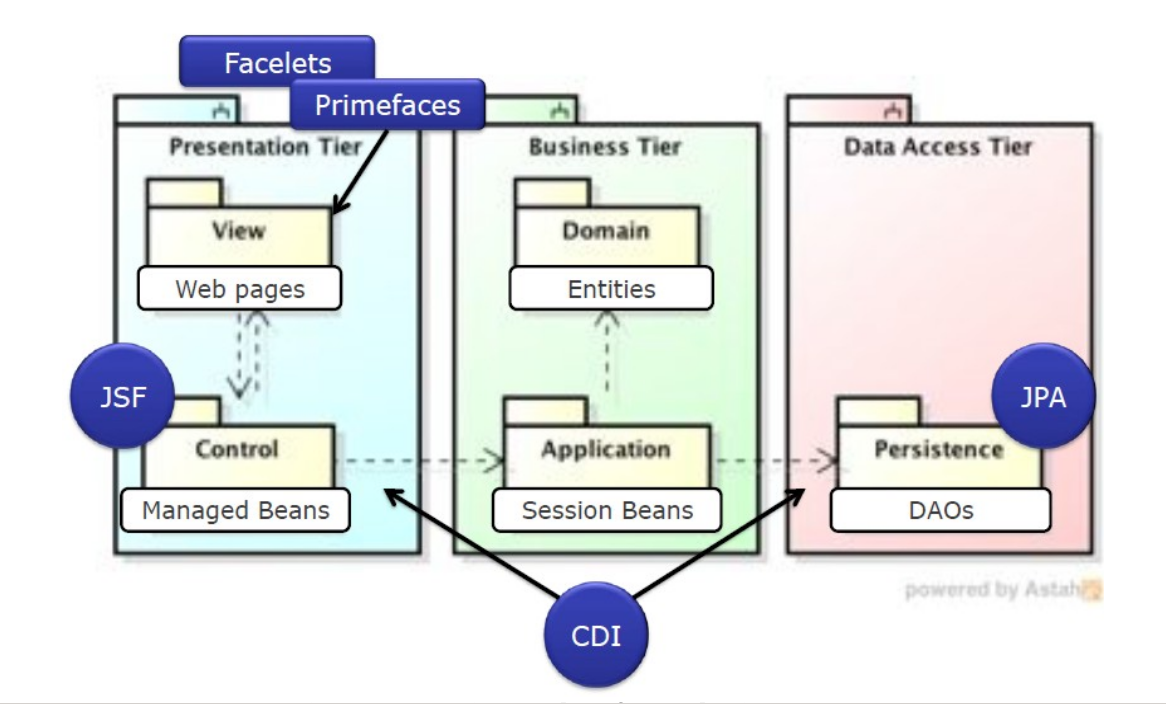
\includegraphics[width=0.9\textwidth]{figuras/arquitetura.png}
  \caption{Arquitetura de Software do Sistema~\cite{lima-pg15}}
  \label{figura-arquitetura}
\end{figure} 



A Figura~\ref{figura-modulos} apresenta a subdivisão de cada módulo nas camadas descritas acima, a saber a Camada de Apresentação (\texttt{control}), Camada de Negócios (\texttt{domain} e \texttt{application}) e Camada de Acesso a Dados (\texttt{persistence}).



\begin{figure}[h]
  \centering
  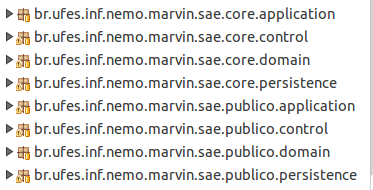
\includegraphics[scale=0.6]{figuras/modulos.png}
  \caption{Subdivisão dos módulos \texttt{sae.core} e \texttt{sae.public} de acordo com a arquitetura de software.}
  \label{figura-modulos}
\end{figure} 





%===================================================================================================================
%									Camada de Apresentação
%===================================================================================================================
\section{Camada de Apresentação}

As funcionalidades criar, visualizar, editar e excluir (abreviadas de CRUD, do inglês \textit{create, read, update and delete}), seguem um mesmo fluxo de execução e de interação com o usuário. Tais funcionalidades são similares para todos os casos de uso cadastrais devido a utilização da ferramenta nemo-utils. Esse fluxo de execução similar é representado na Figura~\ref{figura-modelo-view-crud} através de um modelo de apresentação genérico.

\begin{figure}[h]
  \centering
  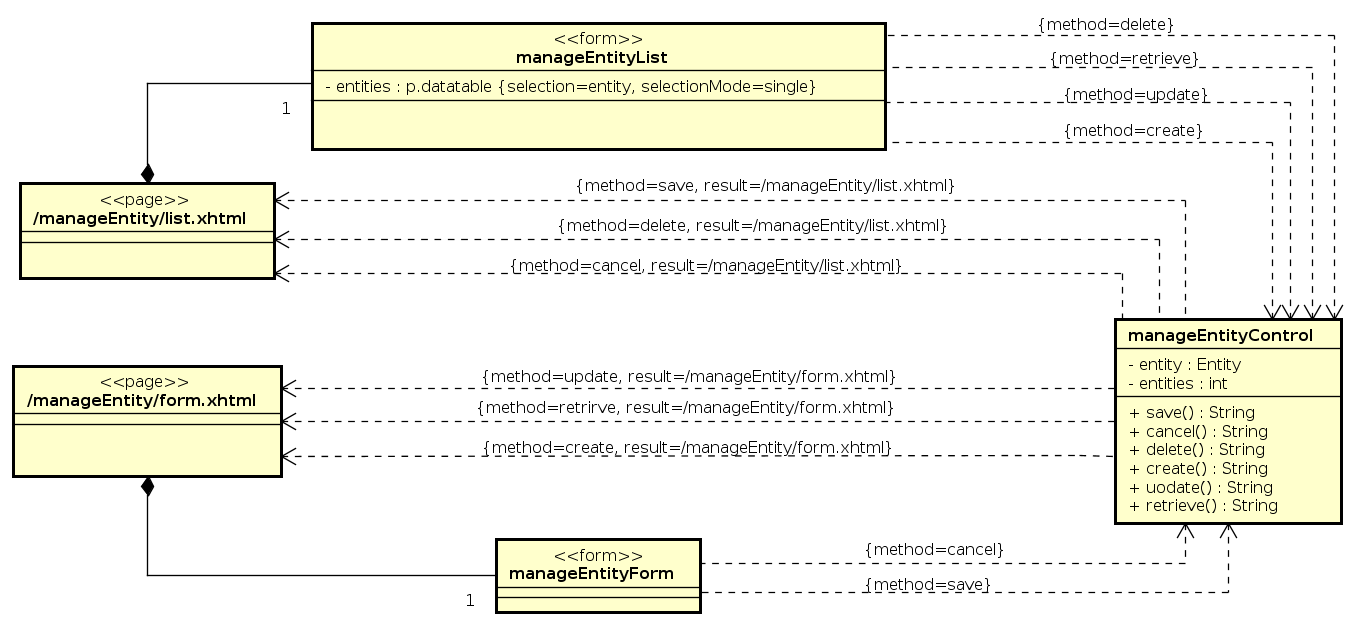
\includegraphics[width=1\textwidth]{figuras/modelocrud}
  \caption{Modelo de Navegação de um CRUD nemo-utils, usado como base para funcionalidades dos cadastros do sistema SAE~\cite{lima-pg15}.}
  \label{figura-modelo-view-crud}
\end{figure} 


Para os casos de uso que apresentam funções diferentes de apenas as básicas de cadastro, o modelo de navegação mostrado anteriormente não pode ser aplicado. Segue na Figura~\ref{figura-modelo-view-analisar-depoimento} o modelo de navegação para o fluxo \emph{Avaliar Depoimento} do caso de uso \emph{Gerenciar Depoimentos}, e na Figura~\ref{figura-modelo-view-consultar-depoimento} o modelo de navegação para o caso de uso \emph{Consultar Depoimentos}.

\begin{figure}[h]
  \centering
  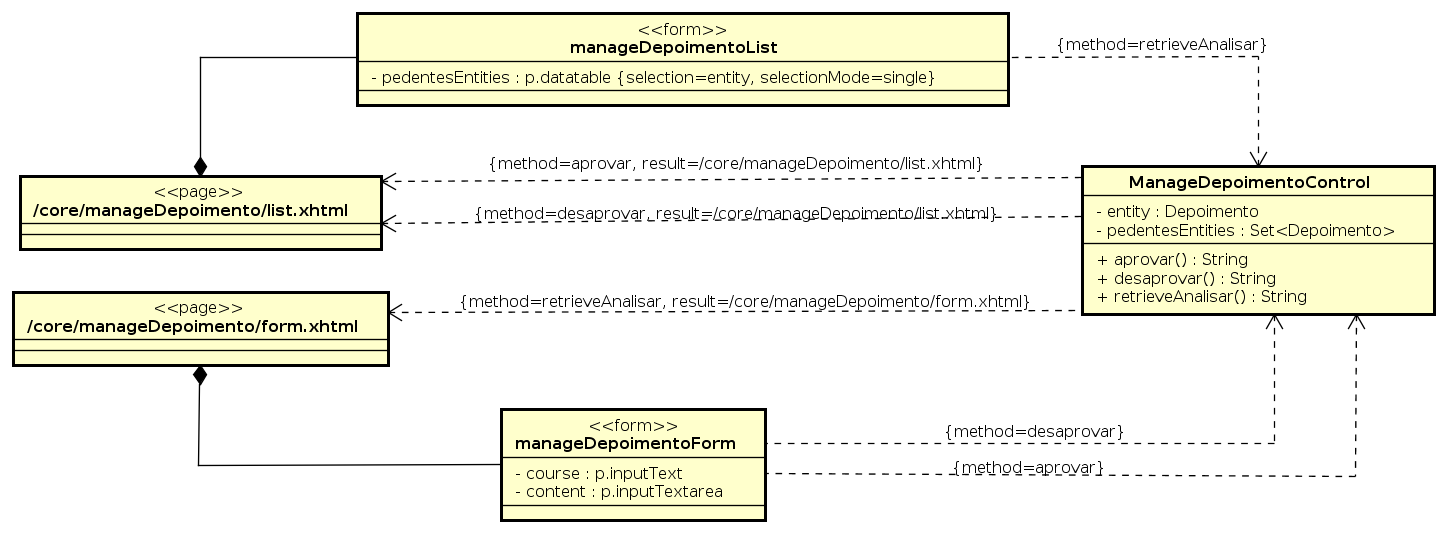
\includegraphics[width=1\textwidth]{figuras/analisarDepoimento}
  \caption{Modelo de Navegação - Avaliar Depoimento.}
  \label{figura-modelo-view-analisar-depoimento}
\end{figure}

\begin{figure}[h]
  \centering
  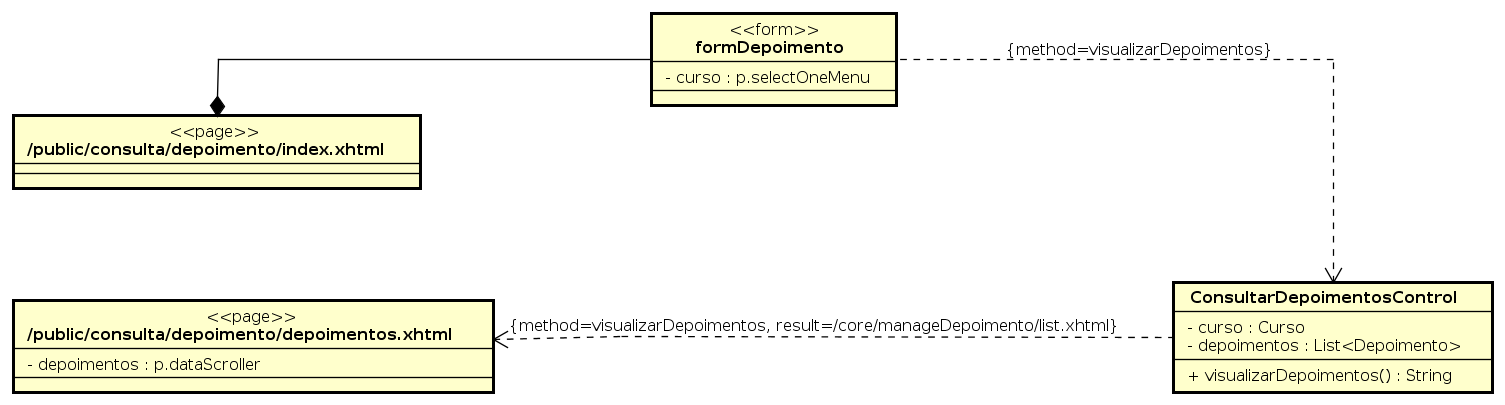
\includegraphics[width=1\textwidth]{figuras/consultarDepoimento}
  \caption{Modelo de Navegação - Consultar Depoimento.}
  \label{figura-modelo-view-consultar-depoimento}
\end{figure} 



%===================================================================================================================
%									Camada de Negócios
%===================================================================================================================
\section{Camada de Negócios }

\subsection{Dominio}
Diferente da abordagem original do FrameWeb original proposto em 2007, todos os atributos que são não nulos tiveram a \textit{tag} \texttt{not null} omitida e os que são nulos tiveram a tag \texttt{null} acrescida de forma a diminuir a poluição visual com repetições desnecessárias no diagrama.

Todas as classes de domínio estendem \texttt{PersistentObjectSupport} do pacote nemo-utils, sendo que essa herança não é mostrada nos diagramas com o intuito de não poluí-los com várias associações.

A Figura~\ref{figura-modelo-dominio-core} mostra o Modelo de Domínio para o módulo \textit{sae.core} e na Figura~\ref{figura-modelo-dominio-publico} o modelo de domínio para o módulo \textit{sae.public}.

\begin{figure}[h]
  \centering
  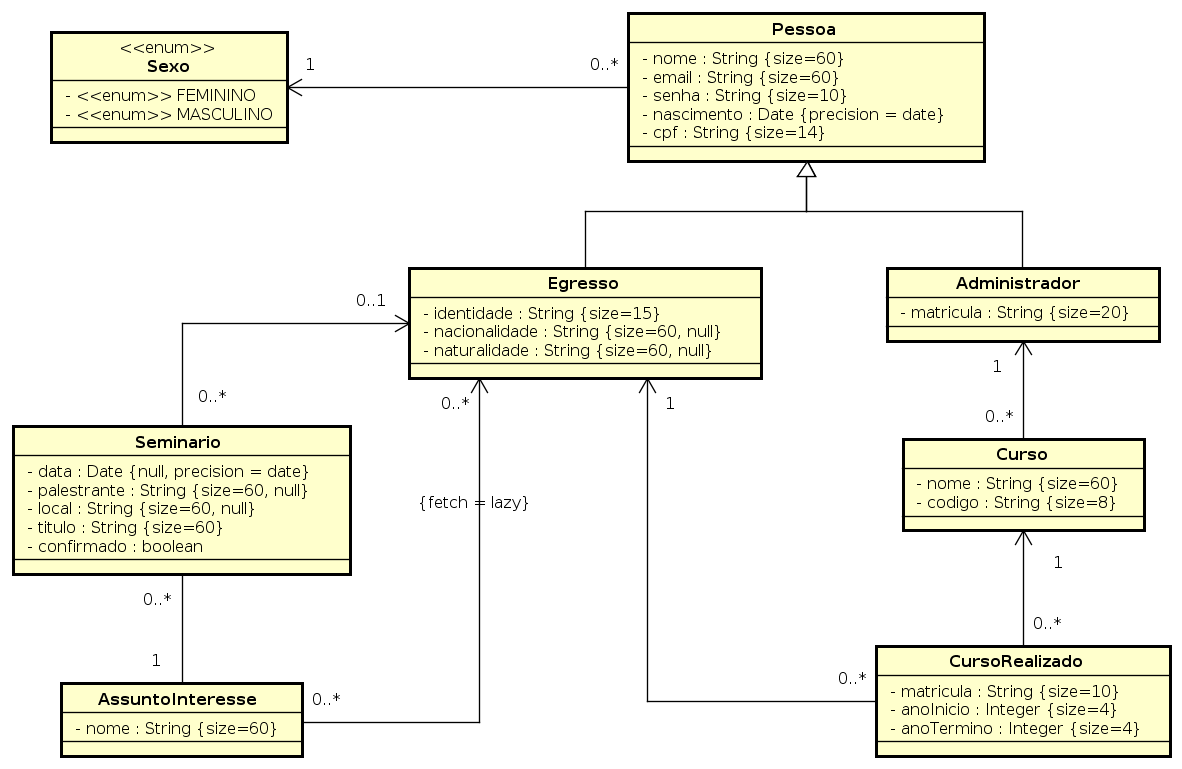
\includegraphics[width=1\textwidth]{figuras/fig-projeto-core-modelo-dominio}
  \caption{Modelo de Domínio do SAE para o módulo \textit{sae.core}.}
  \label{figura-modelo-dominio-core}
\end{figure} 
	
	
\begin{figure}[!h]
  \centering
  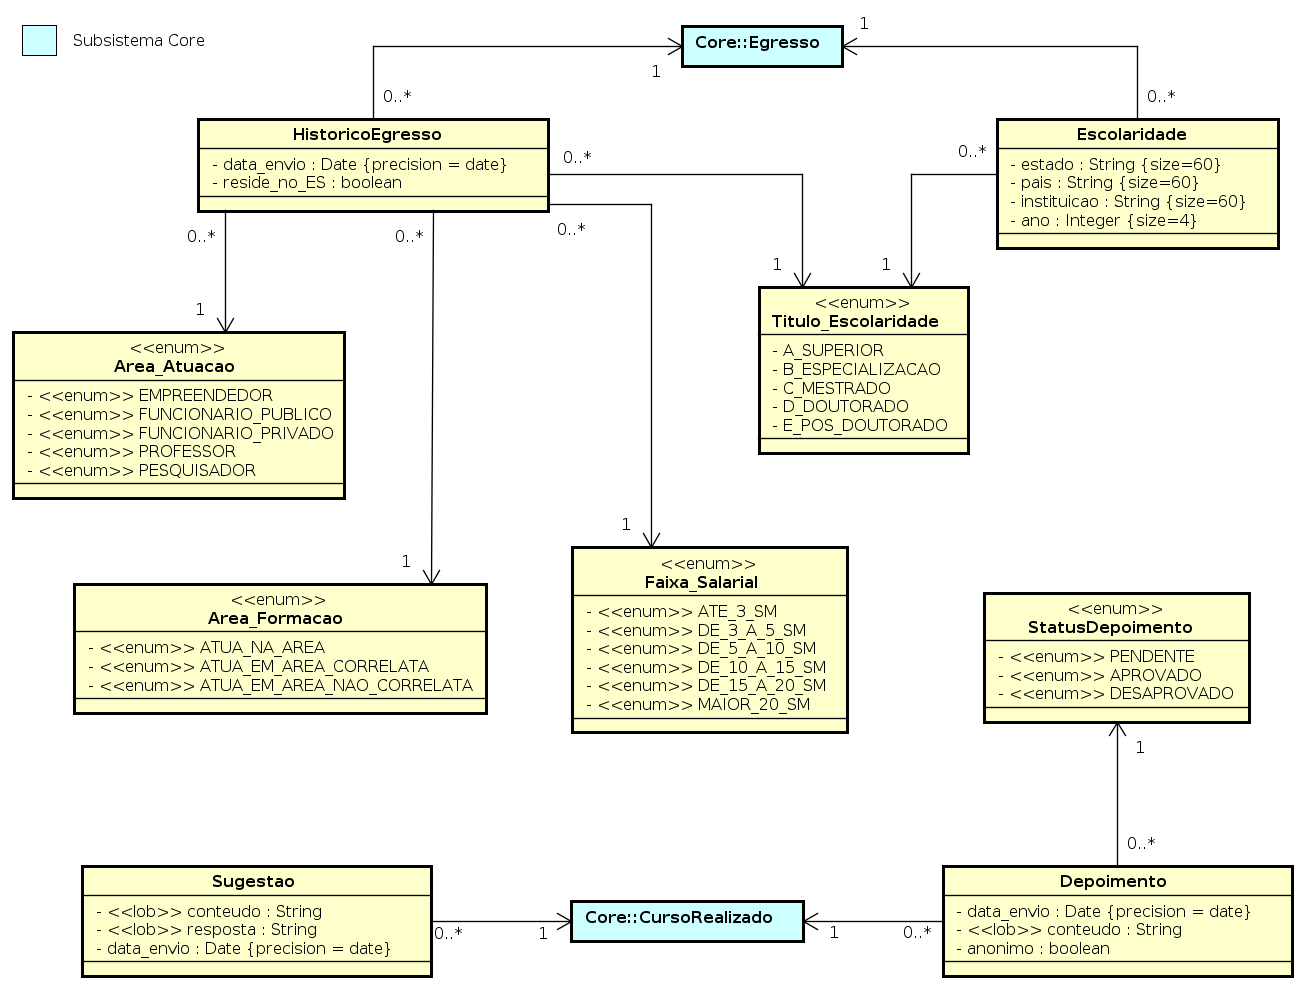
\includegraphics[width=1\textwidth]{figuras/modelodominiopublico.png}
  \caption{Modelo de Domínio do SAE para o módulo \textit{sae.public}.}
  \label{figura-modelo-dominio-publico}
\end{figure} 



Uma observação a ser feita é que classes com potencial de ser comuns a todos os módulos a serem desenvolvidos farão parte do pacote core do Marvin, assim as classes Administrador, Egresso e Curso farão parte deste pacote.







\newpage
\subsection{Aplicação}
Todas as classes de aplicação que são de casos de uso cadastrais estendem de \texttt{CrudServiceBean} do pacote nemo-utils, porém com uma pequena alteração, foi adicionado a classe uma anotação \texttt{@PermitAll} para poder realizar o controle de segurança, tal classe está representada na Figura~\ref{figura-modelo-aplicacao-generico} de forma genérica. Da mesma forma dos diagramas anteriores essa herança não é mostrada no diagrama com o intuito de não poluir o diagrama com várias associações. 

Os casos de uso não cadastrais Confirmar Seminário e Convidar Palestrante, devido sua baixa complexidade e sua alta relação com o caso de uso gereciar seminário, foram adicionados dentro de \texttt{ManageSeminario}.

\begin{figure}[!h]
  \centering
  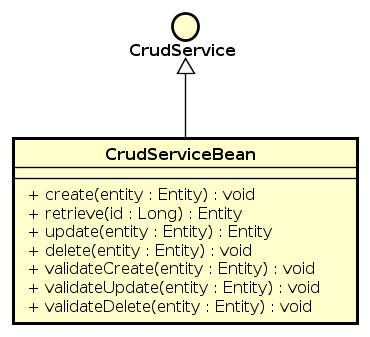
\includegraphics[scale=0.45]{figuras/crudservicebean.png}
  \caption{Modelo de Aplicação genérica da ferramenta nemo-utils.}
  \label{figura-modelo-aplicacao-generico}
\end{figure}

A Figura~\ref{figura-modelo-aplicacao-core} mostra o modelo de aplicação para o módulo \textit{sae.core} e a Figura~\ref{figura-modelo-aplicacao-publico} representa o modelo de aplicação para o módulo \textit{sae.public}.

\newpage

\begin{figure}[!h]
  \centering
  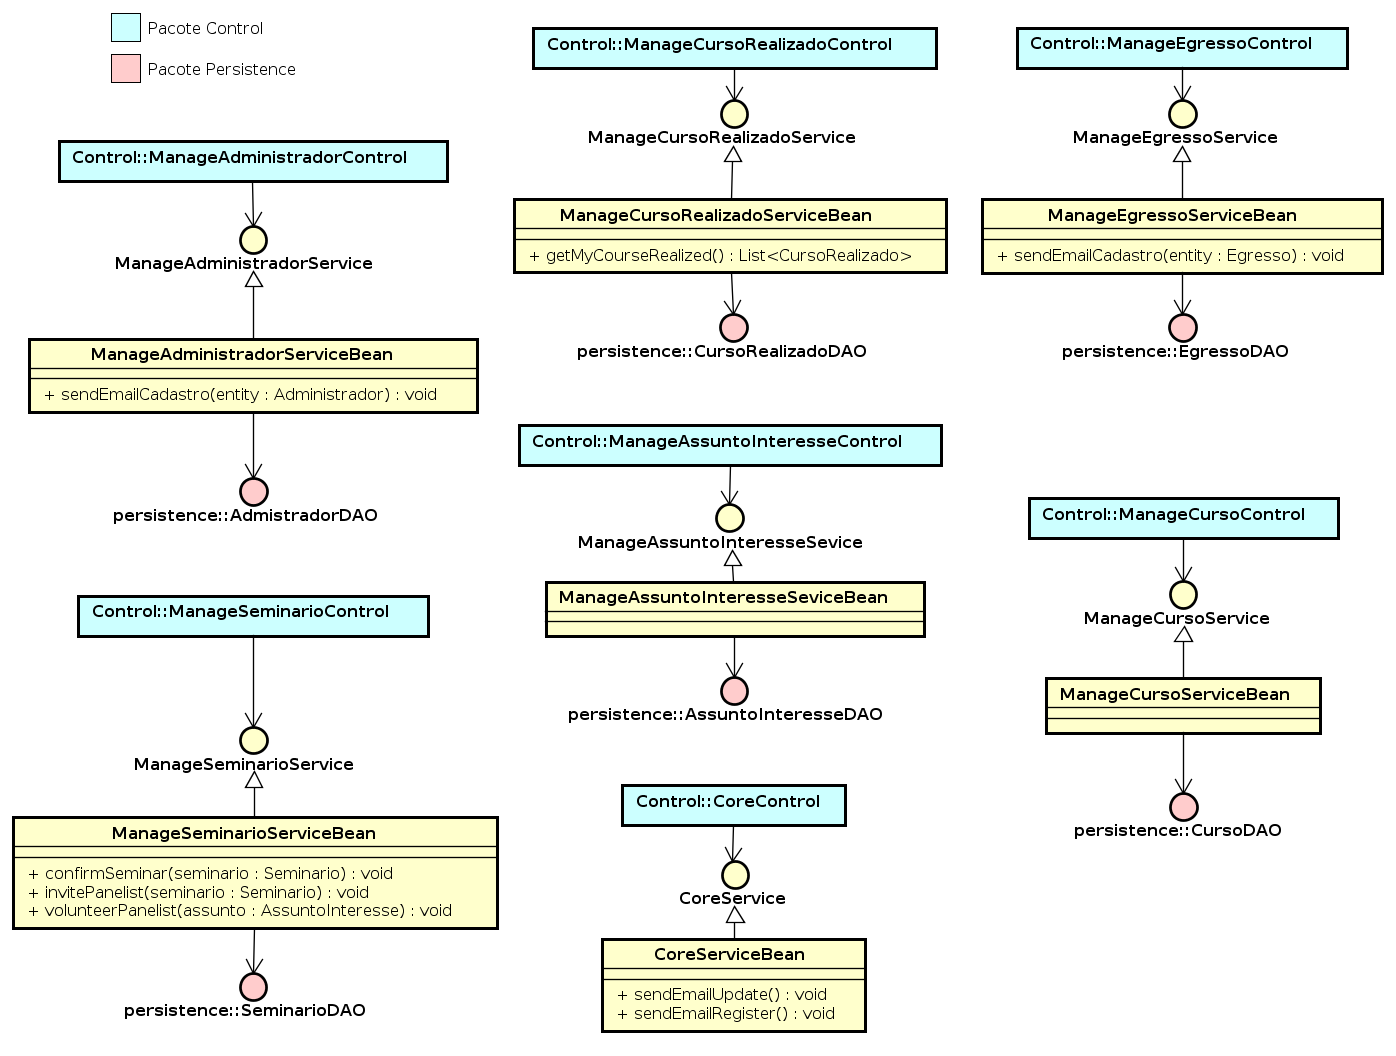
\includegraphics[width=1\textwidth]{figuras/modeloaplicacaocore.png}
  \caption{Modelo de Aplicação do SAE para o módulo \textit{sae.core}.}
  \label{figura-modelo-aplicacao-core}
\end{figure}

\begin{figure}[!h]
  \centering
  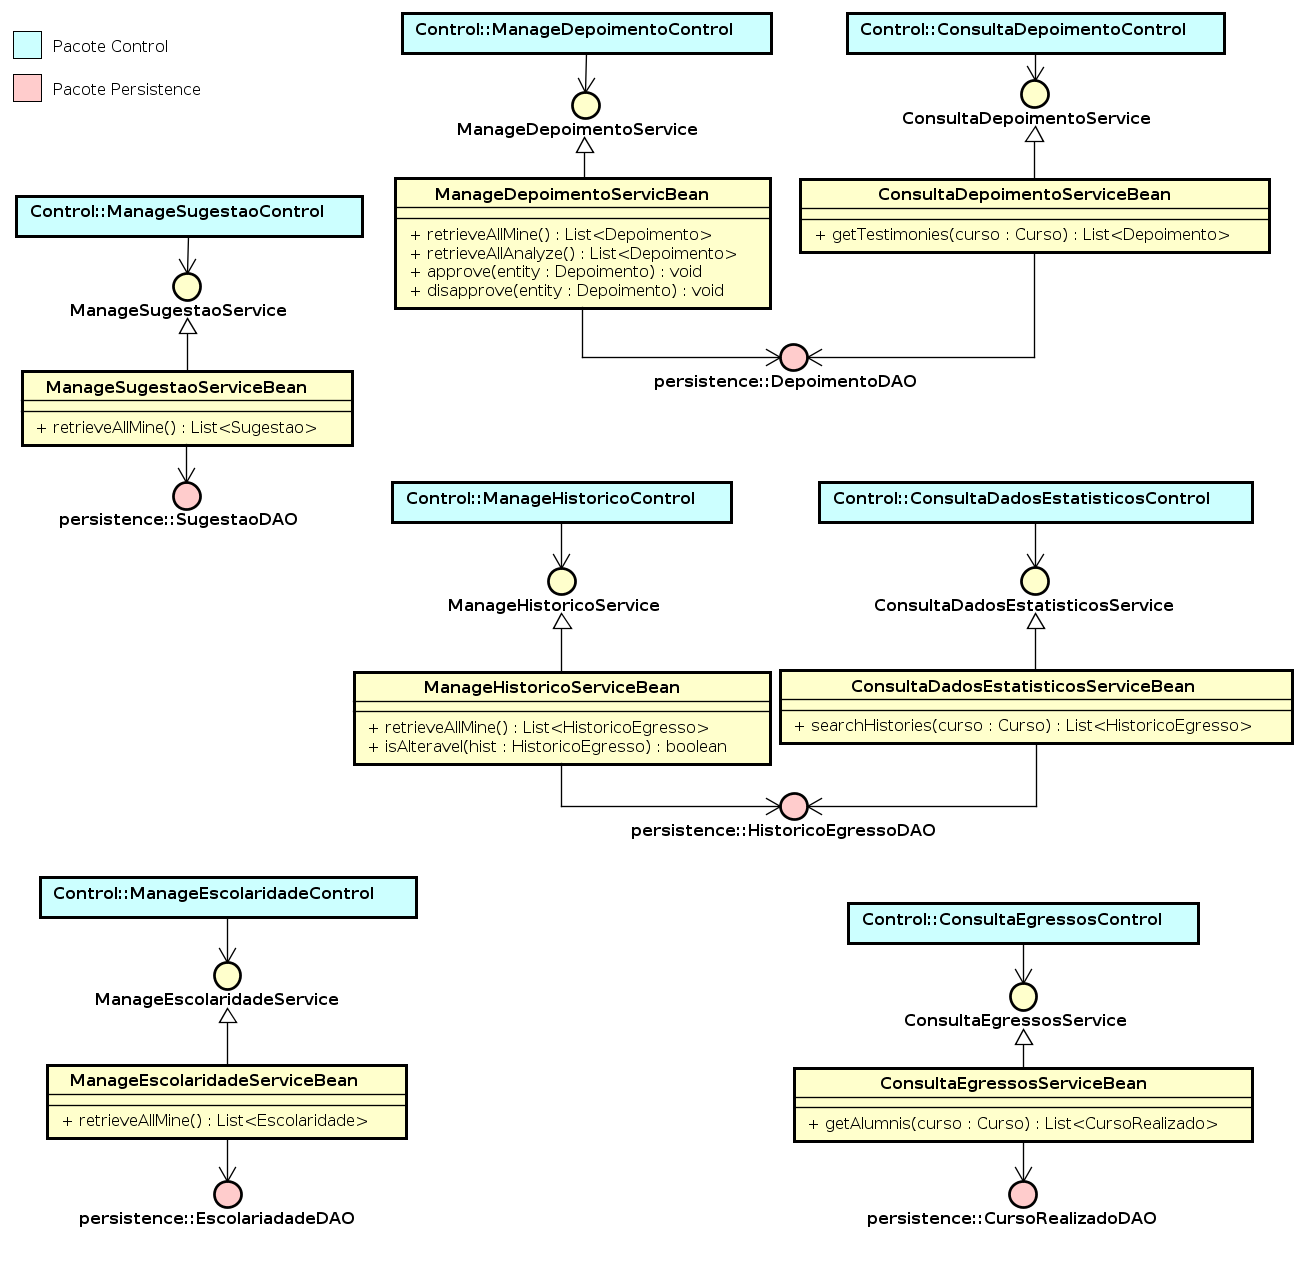
\includegraphics[width=1\textwidth]{figuras/modeloaplicacaopublico.png}
  \caption{Modelo de Aplicação do SAE para o módulo \textit{sae.public}.}
  \label{figura-modelo-aplicacao-publico}
\end{figure}

\newpage




%===================================================================================================================
%									Camada de Acesso a Dados
%===================================================================================================================
\section{Camada de Acesso a Dados}

Nesta seção são apresentados os Modelos de Persistência desenvolvidos para o projeto SAE e que foram usados na implementação do pacote de persistência.


Vale notar que o nome das classes já indica qual tecnologia de persistência foi utilizada, esse sistema de nomenclatura é mais uma sugestão do FrameWeb para simplificar o processo de software. Vale notar também que na Figura~\ref{figura-modelo-persistencia-generico} está representado o diagrama de persistência genérico provido pela ferramenta o nemo-utils. 




\begin{figure}[!h]
  \centering
  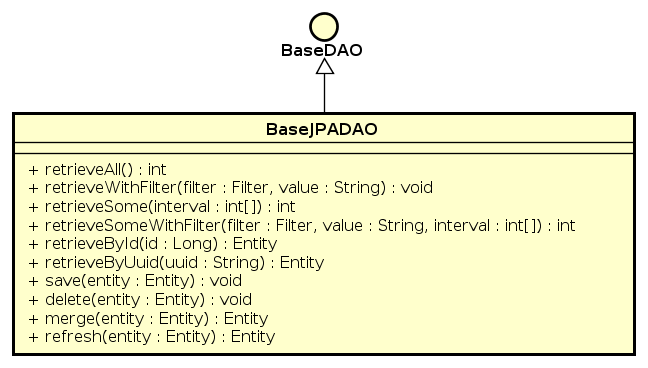
\includegraphics[scale=0.45]{figuras/baseJPADAO.png}
  \caption{Modelo de Persistência genérico da ferramenta nemo-utils.}
  \label{figura-modelo-persistencia-generico}
\end{figure}



Temos na Figura~\ref{figura-modelo-persistencia-core}  o modelo para o módulo \textit{sae.core} e na Figura~\ref{figura-modelo-persistencia-publico} o modelo para o módulo \textit{sae.public}.


\begin{figure}[!h]
  \centering
  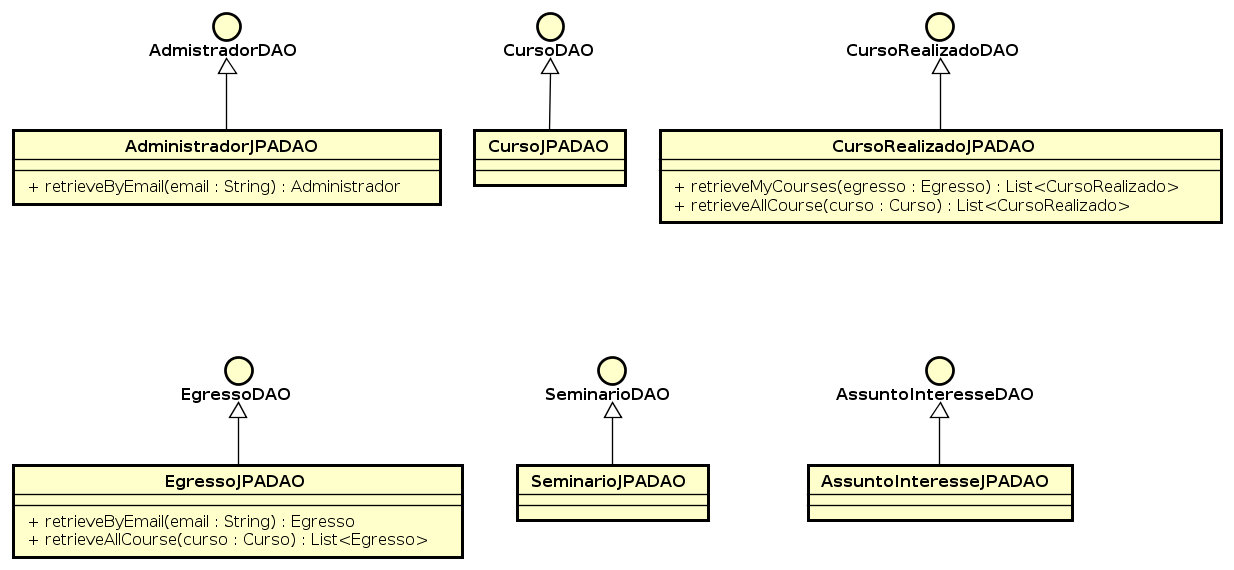
\includegraphics[width=1\textwidth]{figuras/modelopersistencecore.png}
  \caption{Modelo de Persistência do SAE para o módulo \textit{sae.core}.}
  \label{figura-modelo-persistencia-core}
\end{figure}

\newpage

\begin{figure}[!h]
  \centering
  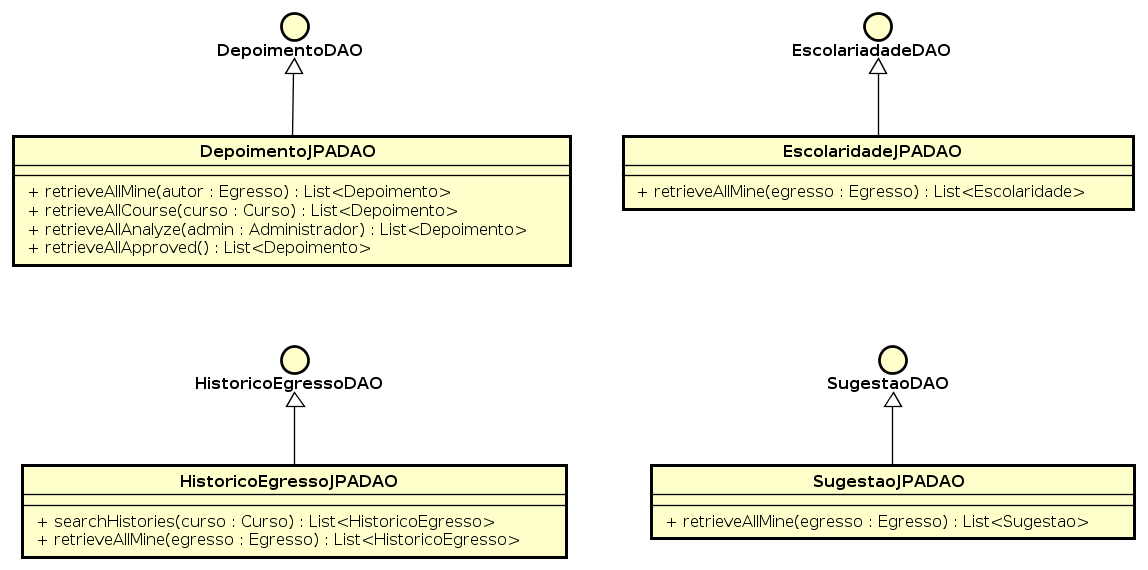
\includegraphics[width=1\textwidth]{figuras/modelopersistencepublico.png}
  \caption{Modelo de Persistência do SAE para o módulo \textit{sae.public}.}
  \label{figura-modelo-persistencia-publico}
\end{figure}




Note que a relação de herança entre os DAOs específicos e o DAO base não é representada explicitamente nos diagramas para evitar poluição visual. Esta também é uma recomendação do FrameWeb, ficando, portanto, o desenvolvedor incumbido de derivar essa relação implicitamente ao analisar o modelo.



